\documentclass[twocolumn]{article}

\usepackage[margin=1in]{geometry}
\usepackage{graphicx}
\usepackage{amssymb}
\usepackage{amsmath}
\usepackage{url}
\usepackage[ruled,vlined]{algorithm2e}

\newcommand{\algohdr}{
\SetKw{BAnd}{and}
\SetKw{BOr}{or}
\SetKw{BIn}{in}
\DontPrintSemicolon \LinesNumbered
}
\newcommand{\ass}{$\leftarrow$\ }

\title{Configuration and Performance Correlation}
\author{Ilari Shafer}
\date{\today}

\begin{document}

\maketitle

\section{Introduction}

In environments where administrators make \textit{configuration changes}, it is often unclear what the effects of such changes are on the system. For instance, suppose an administrator changes a command-line flag to a database server. This flag change turns out to reduce query performance by $50\%$. Currently, the task of associating these two events is very much a manual one, and may involve an administrator examining configuration change logs and time series data from a system such as Nagios or Ganglia. Even when an association between these two sources is made, it is difficult to assess how widespread the 

The methods described below attempt to be a step towards automating this process. They aim to automatically associate configuration changes with changes in time series data. This document describes each of these attempted approaches and indicates where the analysis left off, as either a place to pick up the work or a guide for future efforts.

\section{Background}
Our analysis system should take configuration and performance data, and indicate which configuration changes may have caused changes in performance metrics. This information could take a few forms; here, we focus on answering the question ``which performance changes did a given configuration change produce?'' and (at least initially) ``which configuration changes caused performance changes?''

\subsection{System-independent}
The input to each of these methods are fairly system-agnostic: a set of time series metrics across a number of nodes, and a set of configuration changes. Each of these configuration changes will affect some set of nodes (potentially none).

\subsection{Wikimedia}
At Wikimedia, time series metrics are reported at a granularity of once per day, and different sets of metrics are recorded for different sets of nodes. Here we consider just the set of MySQL database nodes, as the analysis currently does not scale to the entire infrastructure. Configuration is managed with a set of files in Puppet~\cite{puppet}, a declarative configuration management system. To identify the effects of a configuration change, we compile the entire configuration archive at each configuration change, and compute a diff of configuration from one configuration instance to the next.

\section{Methods Attempted}
The goal of all the methods below is to find changes in time series data that may be associated with a given configuration change.

\subsection{Windowing Changepoints}
This approach finds locations in each time series that are likely to be changes, and uses a window after a configuration change to find ``related'' changes. This is a bit clumsy: we do not have an indication of the ``magnitude'' of the change, or a notion of what the window size should be. An implementation is in \texttt{correlate\_v1.r}.

\subsection{Accumulating Changepoint Statistics}
After the first simple attempt, we made the straightforward observation that when looking for time series changepoints, we actually know exactly where to look---the time when the configuration change occurred. 

Looking slightly deeper at changepoint detection algorithms, it turns out some first compute a probability of a changepoint at each timestep, then pick points from the resulting time series (e.g., by thresholding). That is, for each metric, we can compute $P_{\textit{commit},\textit{node},\textit{metric}}$. Currently, it is summed over a window, which may or may not make sense depending upon the test.

The second idea behind this second technique is a heuristic: if a time series change is indeed related to a configuration change, we expect to see time series changes in the metrics on nodes where the change had an effect. Initially I thought of using Jaccard similarity between the set of changed nodes (with a 1 for each time series on that node: $C_{\textit{commit},\textit{node}}$) and metrics with changes, but $P$ is continuous! This method currently uses Pearson's $r$ instead (abusing a mix of notation):
\begin{align*}
r_{commit}=\textup{cor.test}(P_{commit,node,metric}, \\ \{C_{commit,node} \forall metric\})
\end{align*}

\begin{figure}[!t]
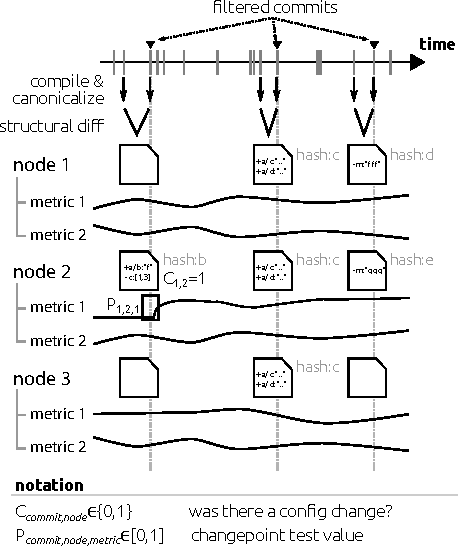
\includegraphics[width=3.2in]{analysis-flow.pdf}
\caption{Flow of changepoint analysis}
\label{fig:analysis-flow}
\end{figure}

The idea is illustrated in Figure~\ref{fig:analysis-flow}, and an implementation is in \texttt{correlate\_v2.r}.

\subsection{Basic Before/After Statistics}
Beyond changepoint detection algorithms, one might wonder if there is something simpler that could also serve as an indicator of change before/after a configuration change. We also experimented with using the mean of a time series before and after the configuration change point and using the mean in a short window before and after a changepoint. These are implemented in \texttt{correlate\_v3.r}.

\section{Output}
The output of all the methods above is a list of configuration changes ranked by how ``likely'' they are to have been the cause of a time series performance change. For each configuration change, there is a ranked list of time series metrics that is currently ordered by 

\section{Future Directions}
A few core challenges caused us to stop pursuing this analysis:

\textbf{Ground truth:} The most critical was the question of where to obtain obtain ground truth for any discoveries. Some of the associations started to make sense to us, but who would identify whether they are correct or not? To establish that our method is producing sensible results (``yes, this configuration change did indeed cause a performance change''), we would need significant additional information. 

One possibility is through documentation in a ticket tracking database that associates the cause or resolution of a problem with a configuration change. Unfortunately, initial exploration along these lines (see Sec.~\ref{sec:scraping}) indicated that this data seems to not exist. 

Another possibility is to replicate a portion of the Wikimedia infrastructure locally and replay configuration changes for a known incoming load. This seems tedious, but is made much more feasible by the fact that Wikimedia provides full Puppet configuration information for all nodes. In theory, it should be possible to use this data to replicate the needed portions of the system for testing purposes.

\textbf{Application-level data:} Although we were able to obtain a significant amount of time series performance data from the Wikimedia foundation, it primarily related to the ``infrastructure''---e.g., CPU usage, free memory, network traffic. Some of these counters extend up to services running on Wikimedia machines (e.g., MySQL active transactions on database nodes). However, the most interesting and useful data from the perspective of diagnosis is information about application performance---for instance, request latency or function execution time. This data does exist, and we have determined how to obtain it, but it is currently kept internal to Wikimedia for technical reasons.

\textbf{Methodology Changes:} Beyond these critical high-level problems, there are a number of knobs in the technique itself to twiddle. We have not yet twiddled these, as resolving some of the problems above is a key first step. That is, some of these could be parameters to explore in an evaluation, but without ground truth it is difficult to tell whether changing them is having an effect.
\begin{itemize}
\item What should we use as the changepoint probability metric? Our initial choice of technique assumes that we are searching for changepoints in normally-distributed data. This assumption is clearly invalid.
\item What should we for accumulating $P$ (e.g., the choice of window size)? Furthermore, should the window weight all points equally, or should there be some decay? Exploration here could help identify effects such as spikes, steps, delayed performance effects, or slow ramps in time series data.
\item What should we use for correlation between configuration changes and metric change strength? Choices here include the technique itself, and going beyond change presence/absence and distinguishing between different change signatures (see \textsf{hash:*} example in Figure~\ref{fig:analysis-flow}).
\end{itemize}

\appendix

\section{Implementation Detail}
For the reader interested in extending this analysis, this section adds a bit more detail on the contents of the code repository, and how to run the system.

\subsection{Scraping Wikimedia Data}
\label{sec:scraping}
There are three sources of data at Wikimedia that the analysis tools collect:

\textbf{Configuration changes:} configuration changes are cloned from Wikimedia's public bug repository at \url{https://github.com/wikimedia/operations-puppet}.

\textbf{Time series performance data:} this is scraped from Wikimedia's public Ganglia page. Run \texttt{scrape.py download} to collect the data; it will be written to a directory named \texttt{timeseries}.

\textbf{Bug database:} this tool scrapes Wikimedia's public Bugzilla repository~\cite{bugzilla} for all bugs in the system and downloads their contents to a directory named \texttt{bugs}. As of the collection performed for the latest analysis, there were 55124 bugs. For the purposes of this analysis, we are only interested in bugs which potentially refer to configuration changes. To filter down to this subset, we first only consider bugs which have an associated code change in Wikimedia' Gerrit code review system\cite{gerrit} (there are 2590 of these), and further, only ones that match changes in the Puppet configuration repository (there are 80 of these). Of the 80 that match configuration-related commits, only one matched a commit that had a configuration diff\footnote{\url{https://github.com/wikimedia/operations-puppet/commit/20f9f94f19c94b6574f1eb27ac13ab97d9891dcb}}.

\subsection{Computing Configuration Diffs}
To obtain diffs of Puppet configuration for each change, we use a bisection search that starts at the first and last commits in the repository, and narrows until it finds an interval over which there are no changes. To compute meaningful diffs, each point of the search compiles the configuration repository down to the ``catalogs'' that would be sent to each node. Slightly more formally, the process looks like:

\begin{algorithm}
\algohdr
\KwData{List of commits $C$}
\KwResult{(side effect) diffs computed by ComputeDiff}
\BlankLine
diff \ass ComputeDiff(C[0], C[C.length-1]) \\
\If{\textup{diff} \BAnd \textup{C.length \textgreater\ 1}}{
	midpt \ass C.length / 2\;
	Diffs(C[0:midpt])\;
	Diffs(C[midpt+1:C.length-1])
}
\caption{Diffs}
\label{alg:cut1}
\end{algorithm}

this is implemented in \texttt{differ.py:245} (\texttt{run\_bisect}). There are other options available for computing diffs: run over only commits that match a filter (\texttt{run\_filtered}) or run a single commit for testing purposes (\texttt{run\_single\_commit}). One other detail is that 

To run the pipeline that computes all configuration diffs, run \texttt{differ.py} with no arguments. We have built a Puppet repository that will set up the compilation on a cluster and a set of scripts to run it, as the full compile is lengthy\footnote{A compile of all changes using the bisection approach across 222 database nodes takes a few days on a cluster of 10 nodes, and a compile across all nodes took a couple weeks on a cluster of 20 nodes}.

\begin{thebibliography}{9}
\bibitem{changepoint} R Package ``changepoint.'' \url{http://cran.r-project.org/web/packages/changepoint/changepoint.pdf}
\bibitem{puppet} Puppet Labs Puppet. \url{http://puppetlabs.com/}
\bibitem{gerrit} Wikimedia Gerrit. \url{https://gerrit.wikimedia.org/r/}
\bibitem{bugzilla} Wikimedia Bugzilla. \url{https://bugzilla.wikimedia.org/}
\end{thebibliography}

\end{document}